\documentclass{article}

\renewcommand{\familydefault}{\sfdefault}  %serifenlose Schrift
\usepackage{helvet} % Schrift: Helvetica


\usepackage{graphicx,graphics,tikz}
\usepackage{amsmath}
\usepackage{amsthm}
\usepackage{xcolor}
\usepackage{amsfonts}
\usepackage{amssymb}
\usepackage{marvosym} % to be able to show male and female symbols with: \Female and \Male
\usepackage{gensymb}
\usepackage[graphics,tightpage,active]{preview}
\PreviewEnvironment{tikzpicture}
\newlength\imagewidth
\newlength\imagescale

\begin{document}

%\pgfmathsetlength{\imagewidth}{10cm} % desired displayed width of image
%\pgfmathsetlength{\imagescale}{\imagewidth/2000} % pixel width of image
% adjust scale of tikzpicture (and direction of y) such that pixel
% coordinates can be used for drawing overlays:
\usetikzlibrary{backgrounds}

\begin{tikzpicture}%[x=\imagescale,y=-\imagescale]

\begin{scope}[xshift=25cm,yshift=-10cm]


\begin{scope}[yshift=-0cm]

\node [scale=1.5,text width=15cm, text centered] at (-8.5cm,-0.6cm) {Species};
\node [scale=1.5,text width=15cm, text centered] at (-1cm,-0.6cm) {Range-limiting factors};
\node [scale=1.1,text width=15cm, text centered,rotate=90] at (-12cm,-5cm){TEMPERATE REGION};
\node [scale=1.1,text width=13cm, text centered,rotate=90] at (-12cm,-11.3cm){ARCTIC REGION};


\begin{scope}[yshift=-0.2cm]
\node (Fs) [scale=1,draw=white, ultra thick,inner sep=0pt,outer sep=0pt] at (-8.5cm,-2.1cm)
  {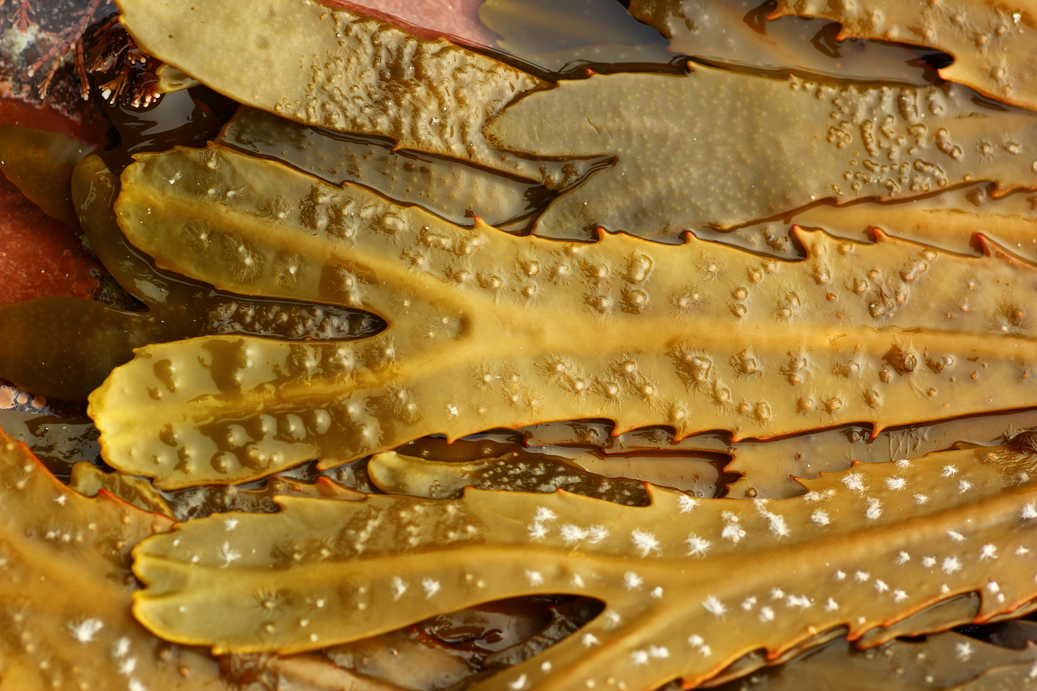
\includegraphics[width=3cm]{IMG_1667_r.png}};
\node [scale=1,text width=8cm, text centered] at (-8.5cm,-3.27cm) {\textit{Fucus serratus}};


\begin{scope}[yshift=-2.5cm]
\node (Fs) [scale=1,draw=white, ultra thick,inner sep=0pt,outer sep=0pt] at (-8.5cm,-2.1cm)
  {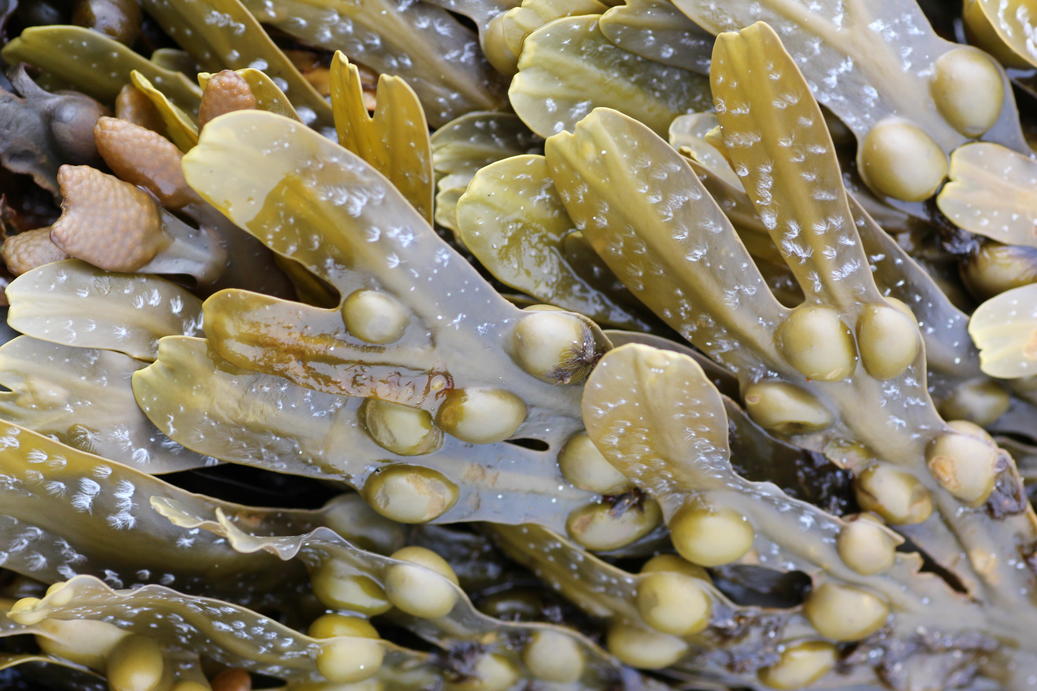
\includegraphics[width=3cm]{IMG_1498_r.png}};
\node [scale=1,text width=8cm, text centered] at (-8.5cm,-3.27cm) {\textit{Fucus vesiculosus}};

\end{scope}

\begin{scope}[yshift=-5cm]
\node (Fs) [scale=1,draw=white, ultra thick,inner sep=0pt,outer sep=0pt] at (-8.5cm,-2.1cm)
  {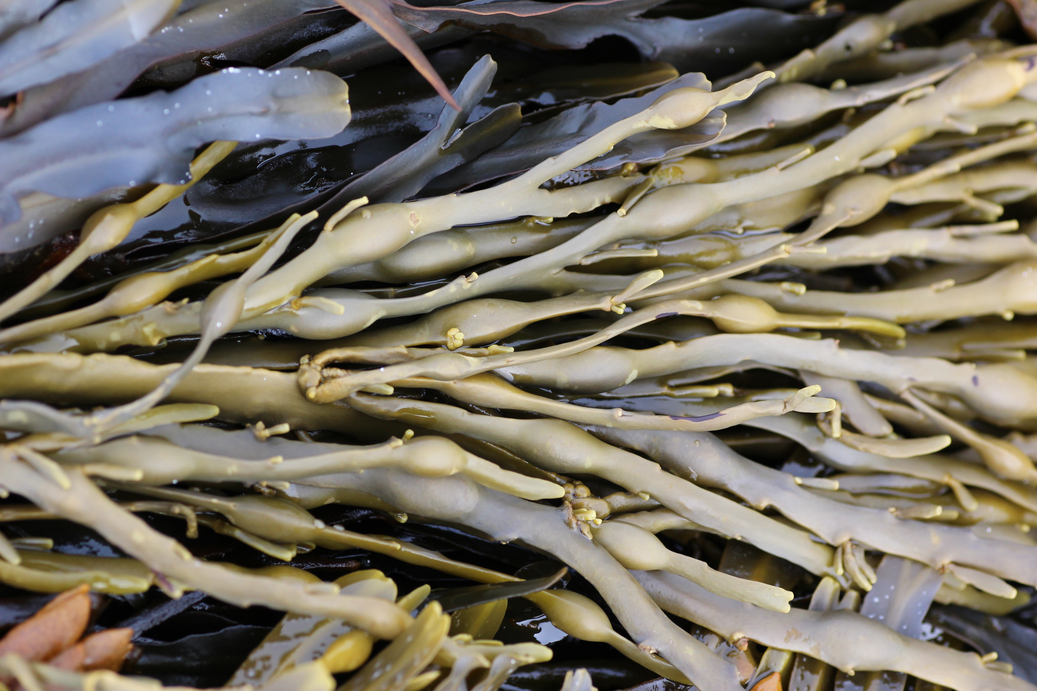
\includegraphics[width=3cm]{IMG_1503_r.png}};
\node [scale=1,text width=8cm, text centered] at (-8.5cm,-3.27cm) {\textit{Ascophyllum nodosum}};


\end{scope}


\begin{scope}[yshift=-8cm]
\node (Fs) [scale=1,draw=white, ultra thick,inner sep=0pt,outer sep=0pt] at (-8.5cm,-2.1cm)
  {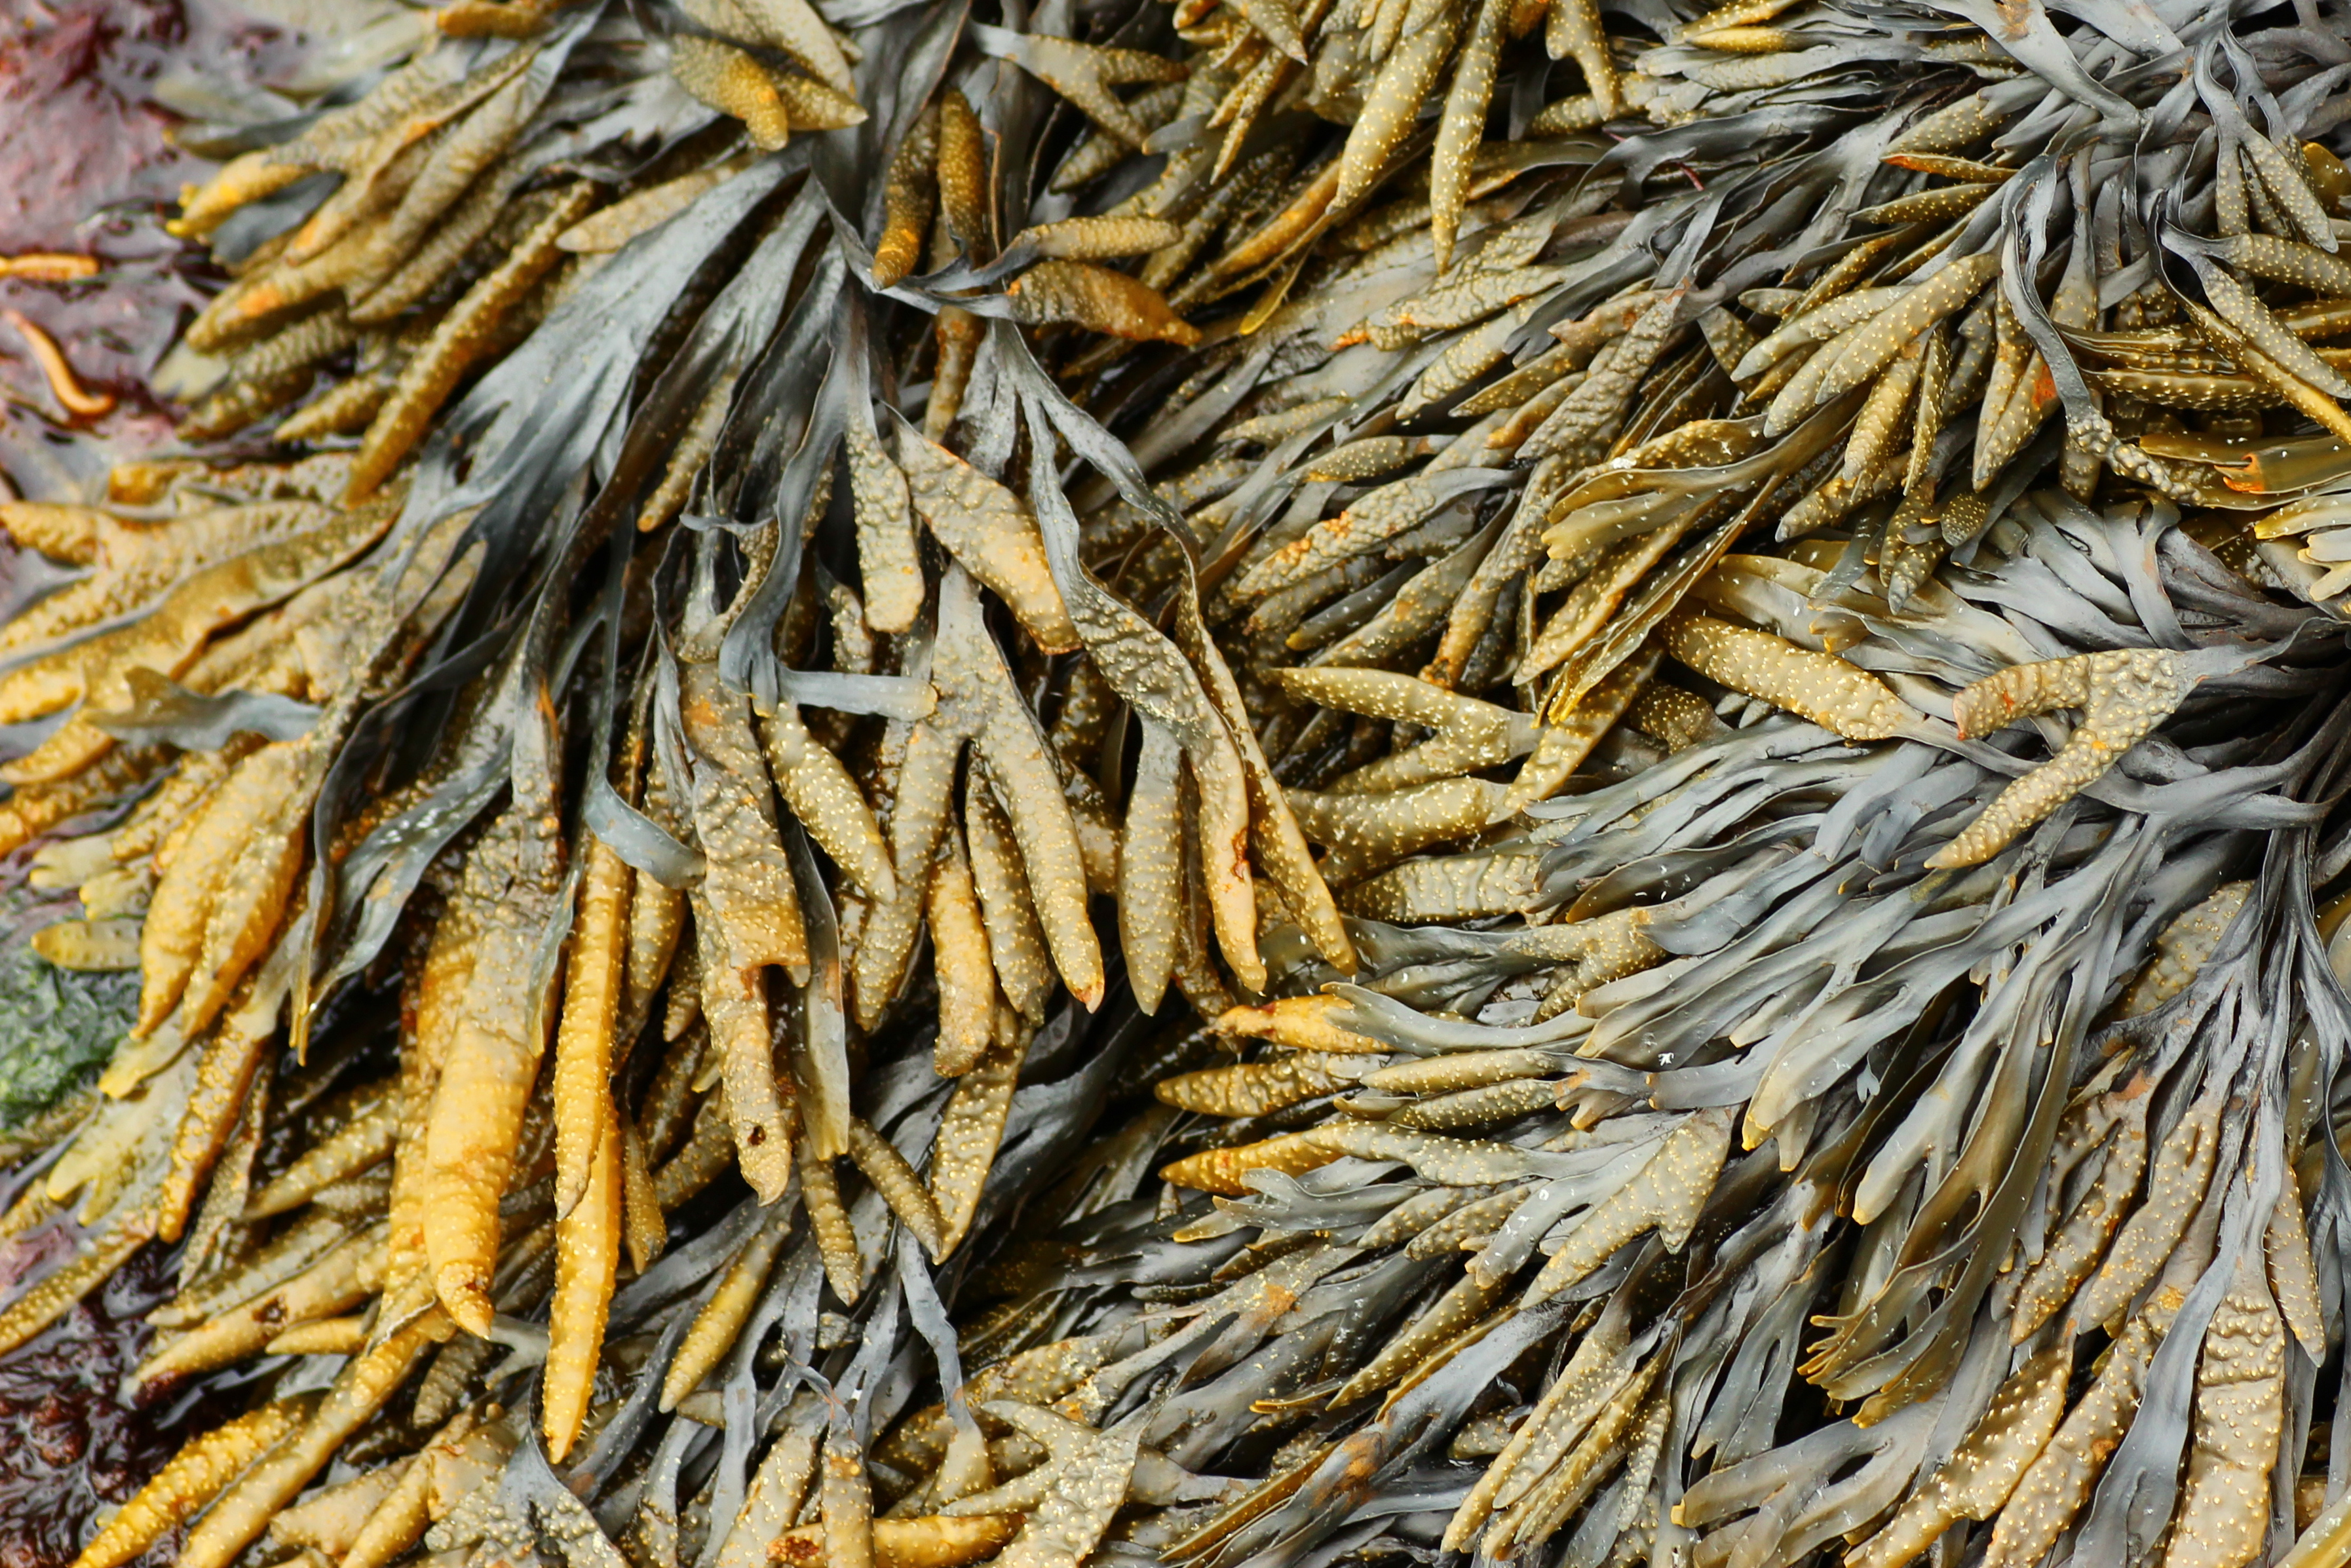
\includegraphics[width=3cm]{IMG_4500_cropped.JPG}};
\node [scale=1,text width=8cm, text centered] at (-8.5cm,-3.27cm) {\textit{Fucus distichus}};


\end{scope}

\end{scope}
\draw [dashed] (-10cm,-8.75cm) -- (2cm,-8.75cm);

\begin{scope}[xshift=-0.65cm]
\node [scale=1,text width=20cm, anchor=west,rotate=80] at (-2.9cm,-15cm) {Minimum \textcolor{red}{SST} ($\degree C$)};
\draw [fill=black] (-2.3cm,-2.5cm) circle (0.1cm);
\draw [fill=black] (-2.3cm,-5cm) circle (0.1cm);
\draw [fill=black] (-2.3cm,-7.5cm) circle (0.1cm);
\draw [dashed] (-2cm,-1.5cm) -- (-2cm,-11cm);

\begin{scope}[xshift=0.6cm]
\node [scale=1,text width=20cm, anchor=west,rotate=80] at (-2.9cm,-15cm) {Mean \textcolor{red}{SST} ($\degree C$)};
\draw [fill=black] (-2.3cm,-2.5cm) circle (0.1cm);
\draw [dashed] (-2cm,-1.5cm) -- (-2cm,-11cm);
\end{scope}

\begin{scope}[xshift=1.2cm]
\node [scale=1,text width=20cm, anchor=west,rotate=80] at (-2.9cm,-15cm) {Maximum \textcolor{red}{SST} ($\degree C$)};
\draw [fill=black] (-2.3cm,-2.5cm) circle (0.1cm);
\draw [fill=black] (-2.3cm,-5cm) circle (0.1cm);
\draw [fill=black] (-2.3cm,-10cm) circle (0.1cm);
\draw [dashed] (-2cm,-1.5cm) -- (-2cm,-11cm);
\end{scope}

\begin{scope}[xshift=1.8cm]
\node [scale=1,text width=20cm, anchor=west,rotate=80] at (-2.9cm,-15cm) {Mean \textcolor{red}{SAT} ($\degree C$)};
\draw [fill=black] (-2.3cm,-7.5cm) circle (0.1cm);
\draw [dashed] (-2cm,-1.5cm) -- (-2cm,-11cm);
\end{scope}

\begin{scope}[xshift=2.4cm]
\node [scale=1,text width=20cm, anchor=west,rotate=80] at (-2.9cm,-15cm) {Min. Diff. Atten. ($m^{-1}$)};
\draw [fill=black] (-2.3cm,-5cm) circle (0.1cm);
\draw [dashed] (-2cm,-1.5cm) -- (-2cm,-11cm);
\end{scope}

\begin{scope}[xshift=3cm]
\node [scale=1,text width=20cm, anchor=west,rotate=80] at (-2.9cm,-15cm) {Mean Salinity ($PSU$)};
\draw [fill=black] (-2.3cm,-7.5cm) circle (0.1cm);
\draw [dashed] (-2cm,-1.5cm) -- (-2cm,-11cm);
\end{scope}

\begin{scope}[xshift=3.6cm]
\node [scale=1,text width=20cm, anchor=west,rotate=80] at (-2.9cm,-15cm) {Mean Nitrate ($\micro mol l^{-1}$)};
\draw [fill=black] (-2.3cm,-10cm) circle (0.1cm);
\draw [dashed] (-2cm,-1.5cm) -- (-2cm,-11cm);
\end{scope}

\begin{scope}[xshift=4.2cm]
\node [scale=1,text width=20cm, anchor=west,rotate=80] at (-2.9cm,-15cm) {Min. Chlorophyll ($mg/m^{3}$)};
\draw [fill=black] (-2.3cm,-10cm) circle (0.1cm);
\draw [dashed] (-2cm,-1.5cm) -- (-2cm,-11cm);
\end{scope}

\begin{scope}[xshift=4.8cm]
\node [scale=1,text width=20cm, anchor=west,rotate=80] at (-2.9cm,-15cm) {Mean Calcite ($mol/m^{3}$)};
\draw [fill=black] (-2.3cm,-10cm) circle (0.1cm);
% \draw [dashed] (-2cm,-1cm) -- (-2cm,-11cm);
\end{scope}
\end{scope}

%\node (2200map) [draw=white, ultra thick,inner sep=0pt,outer sep=0pt] at (-1.5cm,-0.7cm)
%  {\includegraphics[width=2.5cm, bb=85 130 815 670, clip]{2011-12-18-Projection_binary_2200.png}};


%\begin{scope}[shorten <=0.25cm, shorten >=0.25 cm]
%\draw [->, line width=0.03cm] (model) to [out=270,in=90] (2000point);
%\draw [->, line width=0.03cm] (model) to [out=270,in=90] (2100);
%\draw [->, line width=0.03cm] (model) to [out=270,in=90] (2200);
%\end{scope}
\end{scope}

\end{scope}

\end{tikzpicture}


\end{document}